\documentclass[cn,hazy,green,12pt,normal]{elegantnote}

\title{作业2解答}
\author{24Spring 回归分析}
\date{\today}

\usepackage{array}

\usepackage{amsmath, amssymb, bm, color, framed, graphicx, hyperref, mathrsfs, fontspec, geometry, extarrows, amsthm}

\DeclareMathOperator{\e}{\!\!\;\mathrm e}
\DeclareMathOperator{\Cov}{Cov}
\DeclareMathOperator{\Var}{Var}
\DeclareMathOperator{\var}{var}
\DeclareMathOperator{\tr}{tr}
\DeclareMathOperator{\diag}{diag}
\newcommand{\p}{\partial}
\renewcommand{\d}{\mathop{}\!\mathrm{d}}
\newcommand{\MR}{\mathbb R}
\newcommand{\MC}{\mathbb C}
\newcommand{\MF}{\mathbb F}
\newcommand{\MZ}{\mathbb Z}
\newcommand{\MN}{\mathbb N}
\newcommand{\MCF}{\mathscr F}
\renewcommand{\Re}{\operatorname{Re}}
\renewcommand{\Im}{\operatorname{Im}}
\renewcommand{\boldsymbol}{\bm}
\renewcommand{\i}{\mathrm i}

\DeclareMathOperator{\Arg}{Arg}
\DeclareMathOperator{\I}{I}
\usepackage{tkz-euclide}
\numberwithin{equation}{section}
\numberwithin{subsection}{section}

\lstset{
    language=R,
    basicstyle=\ttfamily,
    keywordstyle=\color{blue},
    commentstyle=\color{gray},
    frame=single,
    breaklines=true
}

\begin{document}
\maketitle
\begin{homework}
    设
    \[
    \begin{aligned}
    y_1&=\theta+e_1\\
    y_2&=2\theta-\varphi +e_2\\
    y_3&=\theta+2\varphi +e_3\\
    \end{aligned}
    \]
    其中$\theta,\varphi$为未知参数。$E(e_i)=0,Var(e_i)=\sigma^2,\forall i$,且$e_i$相互独立。

    (a)求$\theta,\varphi$的最小二乘估计$\hat{\theta},\hat{\varphi}$;

    (b)求$\Cov\begin{bmatrix}
        \hat{\theta}\\
        \hat{\varphi}
    \end{bmatrix}$
\end{homework}
\begin{proof}[\solutionname]
   (a) 记\[
    \bm \beta = \begin{bmatrix}
        \theta\\
        \varphi
    \end{bmatrix},\quad \bm y = \begin{bmatrix}
        1&0\\
        2&-1\\
        1&2\\
    \end{bmatrix}\bm \beta +\bm e
    \]
    代入公式即得。

    (b)利用$\Cov(\bm \hat{\beta})=\sigma^2(X^TX)^{-1}$
   
\end{proof}

\begin{homework}
    设\[
    \begin{aligned}
        &y_i=\theta +e_i, \quad i=1,\dots,m\\
        &y_{m+j}=\theta +\varphi +e_{m+j}\quad j=1,\dots,m\\
        &y_{2m+k}=\theta -2\varphi +e_{2m+k},\quad k=1,\dots,n
    \end{aligned}
    \]
    其中$\theta,\varphi$为未知参数,$e_i\quad i.i.d. \sim N(0,\sigma^2)$。

    (a)写出设计阵X

    (b)求$\theta,\varphi$的最小二乘估计$\hat{\theta},\hat{\varphi}$

    (c)证明当m=2n时,$\hat{\theta}$与$\hat{\varphi}$不相关。
\end{homework}
\begin{proof}[\solutionname]
    类似作业7,代入公式求解即可,第三问考虑两者协方差。
\end{proof}

\begin{note}
    具体过程示例: % 改图片符号
    
    \begin{figure}[!htbp]
        \centering
        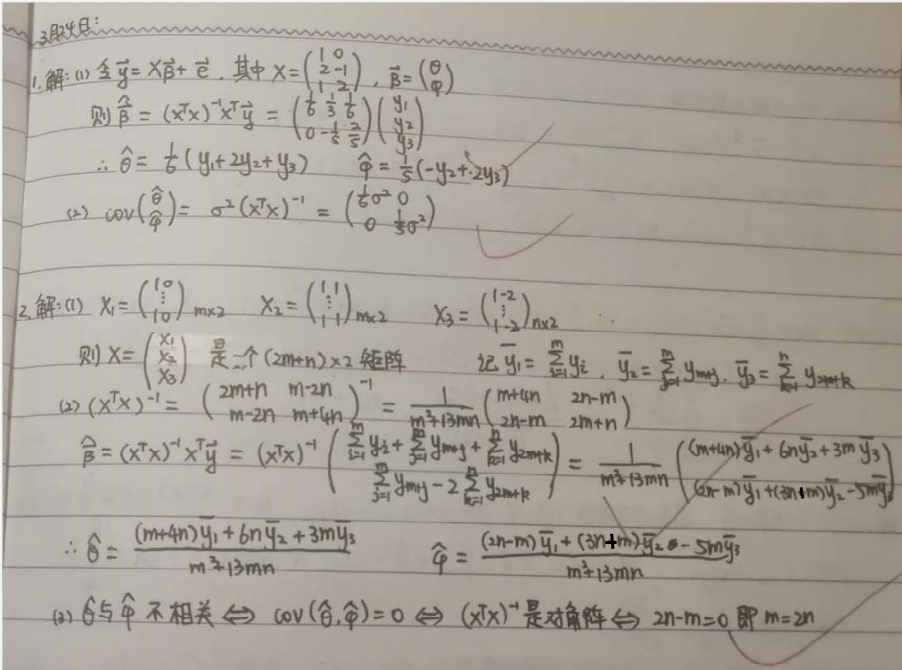
\includegraphics[width=30em]{image/ex2_plt8.png}
    \end{figure} 
    
\end{note}
\begin{homework}
    已知$X\sim N_n(\bm \mu, I_n )$

    (a)求$Y_1=\bm a ^T X$和$Y_2=\bm b^T X$的联合分布,其中$\bm a, \bm b$为$n\times 1$常向量,且不共线。

    (b)若$\bm a^T \bm b=0$,证明$Y_1,Y_2$独立。
\end{homework}

\begin{proof}
    (a) 记$A=\begin{bmatrix}
        \bm a^T\\
        \bm b^T\\
    \end{bmatrix}$行满秩,考虑$\begin{bmatrix}
        Y_1 \\
        Y_2\\
    \end{bmatrix}=AX\sim N_2(A\mu,AA^T)$
    
    (b)从联合分布可知,此时协方差阵为对角阵。多元正态不相关进而独立。
\end{proof}

\begin{note}
    注意各分量服从正态分布,不一定总体服从联合正态分布。比如联合密度
    \[f(x,y)=\dfrac{1}{2\pi} e^{-\frac{1}{2}(x^2+y^2)}\left[ 1-\dfrac{xy}{(x^2+1)(y^2+1)}\right]\]
    边际分布服从标准正态分布。这题不要从分量的角度写,应当整体分析。
\end{note}

\begin{homework}
    设$X\sim N_n(\bm \mu, \Sigma),A$是$n\times n$对称矩阵,证明当$A\Sigma A=A$时,$(X-\bm \mu )^TA(X-\bm \mu)\sim \chi_r^2,r=Rank(A)$
\end{homework}
\begin{proof}
    由于$\Sigma$为正定阵,故$A=A\Sigma A=A\Sigma A^T$半正定
    \newpage
    \begin{figure}[!htbp]
        \centering
        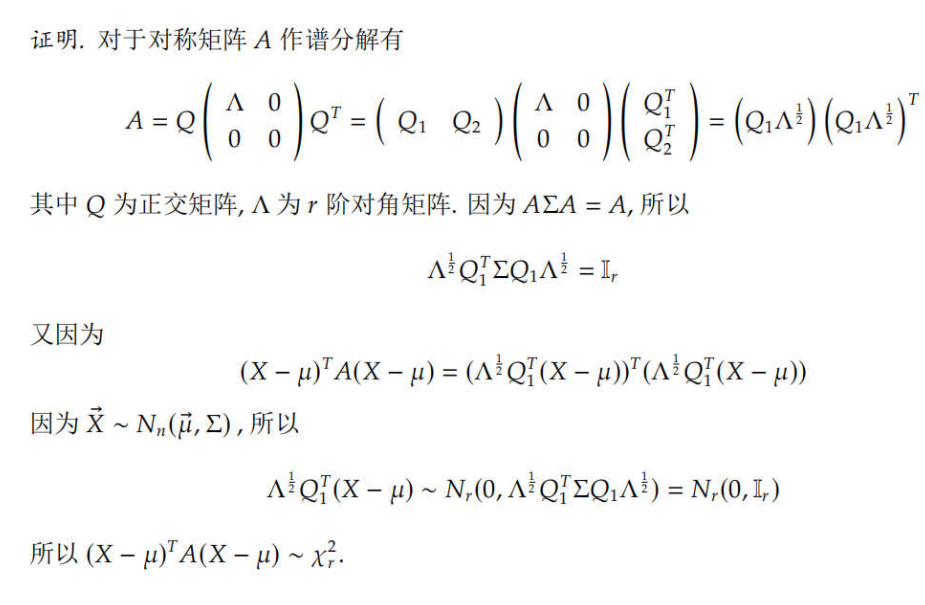
\includegraphics[width=30em]{image/ex1_plt2.png}
    \end{figure}
    
\end{proof}
\begin{note}
    (1)证明中需要说明$\Lambda$对角元大于0。(否则如果有小于0的分量,则没有$\Lambda^{1/2}$,因为不在复数域讨论)

    \noindent (2) 也可以考虑
    $Y=\Sigma^{-\frac{1}{2}}(X-\mu)\sim N(0,I_n)$,\[
    (X-\mu)^TA(X-\mu)=Y^T\Sigma^{\frac{1}{2}}A\Sigma^{\frac{1}{2}}Y\]
    ,并验证$\Sigma^{\frac{1}{2}}A\Sigma^{\frac{1}{2}}$为秩为$r$的投影阵(对称幂等)。
\end{note}
\newpage
\begin{homework}
    对于简单线性回归模型:
    \[y_i=\beta_0+\beta_1x_i+e_i\]满足Gauss-Markov假设,验证通过OLS得到的拟合回归直线其残差平方和
    \[RSS=SYY-\dfrac{(SXY)^2}{SXX}\],
    并证明测定系数$R^2$等于因变量Y与自变量X之间样本相关系数的平方,即
    \[R^2=\dfrac{(SXY)^2}{SXX\cdot SYY}\]
\end{homework}
\begin{proof}[\solutionname]
\end{proof}
    \begin{figure}[!htbp]
        \centering
        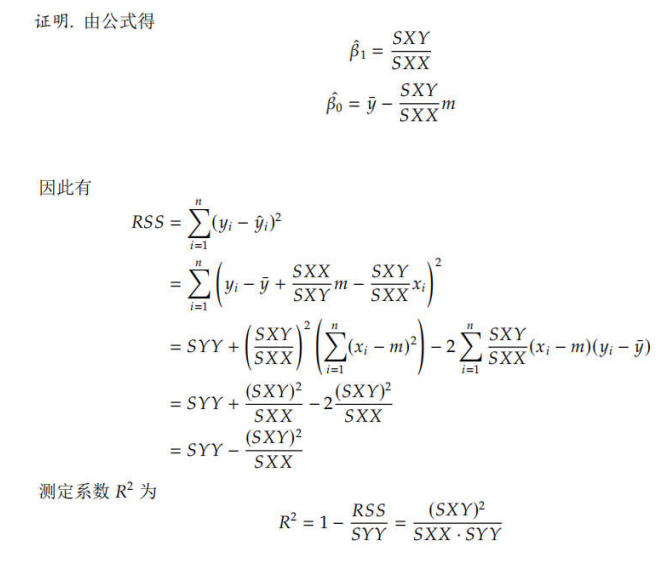
\includegraphics[width=30em]{image/ex2_plt1.png}
    \end{figure}

    解法2:$RSS=||\bm y-\hat{\bm y} ||^2,\quad R^2=\dfrac{SS_{Reg}}{SYY}=\dfrac{||\hat{\bm y}-\bm 1 \Bar{y}||^2}{||\bm y-\bm 1 \Bar{y}||^2}$

    并且有$(\bm y-\hat{\bm y})\perp (\hat{\bm y}-\bm 1 \Bar{y})$,由勾股定理$SYY=SS_{Reg}+RSS$,只需求解$SS_{Reg}$。
    \[SS_{Reg}=||H \bm y - \bm 1 \Bar{y}||^2=||(P_{\bm 1}+P_{X_c})\bm y-\bm 1 \Bar{y}||^2=||P_{X_c}\bm y||^2=\bm y^TX_c(X_c^TX_c)^{-1}X_c^T\bm y=\dfrac{(SXY)^2}{SXX}\]
    代入即得。
\newpage

\begin{homework}
\end{homework} % 题目修改为$y_i=\beta_1 x_{i,1}+\beta_2 x_{i,2}+\dots +\beta_{p-1}x_{i,p-1}+e_i$, 并增加原题目讨论

    \begin{figure}[!htbp]
        \centering
        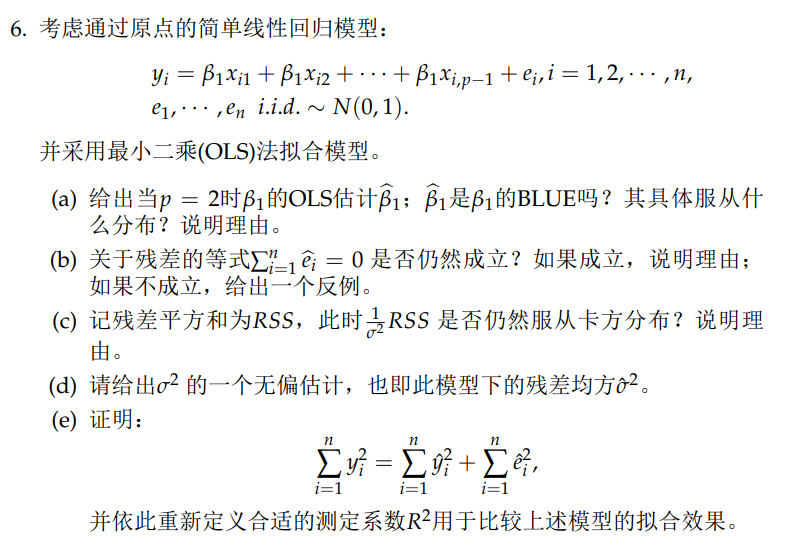
\includegraphics[width=25em]{image/ex2_plt2.png}
    \end{figure}

    此题题目模型改为\[y_i=\beta_1 x_{i,1}+\beta_2 x_{i,2}+\dots +\beta_{p-1}x_{i,p-1}+e_i\]
    改完后(c)(d)两问自由度为n-p+1。这次作业若按照原题目自由度为n-1计算,也算满分。
    
\begin{proof}[\solutionname]
(a):\[\hat{\beta}_1=(X^TX)^{-1}X^Ty = \dfrac{\sum x_iy_i}{\sum x_i^2}\]
由GM定理,$\hat{\beta}_1$为$\beta_1$的BLUE。
\[\hat{\beta}_1=(X^TX)^{-1}X^T(X\beta+e)=\beta+(X^TX)^{-1}X^T e\sim N(\beta,(X^TX)^{-1})= N(\beta,\dfrac{1}{\sum x_i^2})\]
\noindent (b)不成立(因为$\bm 1 \notin P_X$,$\sum \hat{e_i}=\bm 1^T(I_n-P_X)y$不一定为0 )反例比如\[x_1=1,y_1 =0,x_2=2,y_2=1\]
\noindent (c)是,因为
\[\frac{RSS}{\sigma^2} =\frac{1}{\sigma^2}y^T(I_n-H)y=(\frac{e}{\sigma})^T(I_n-H)\frac{e}{\sigma}, \quad rank(I_n-H) = n-(p-1)=n-p+1\]
\[\frac{e}{\sigma}\sim N(0,I_n),\quad I_n-H\text{对称幂等}\Rightarrow \frac{RSS}{\sigma^2}\sim \chi_{n-p+1}^2\]
\noindent (d)由(c)得$\hat{\sigma}^2 = \frac{RSS}{n-p+1}$满足$E[\hat{\sigma}^2]=\sigma^2$

\noindent (e)\[||y||^2=||\hat{y}+(y-\hat{y})||^2,\quad \hat{y}\perp y-\hat{y} \Rightarrow ||y||^2=||\hat{y}||^2+||\hat{e}||^2\]
定义测定系数$R^2 = \dfrac{||\hat{y}||^2}{||y||^2}\in [0,1]$
\end{proof}

\begin{note}
    (1)注意GM定理的使用条件,这里是可以对无截距模型应用的,因为不涉及考察X第一列性质(i.e. $\bm 1$是否属于C(X))。
\end{note}
\newpage
\begin{homework}
\end{homework}
    \begin{figure}[!htbp]
        \centering
        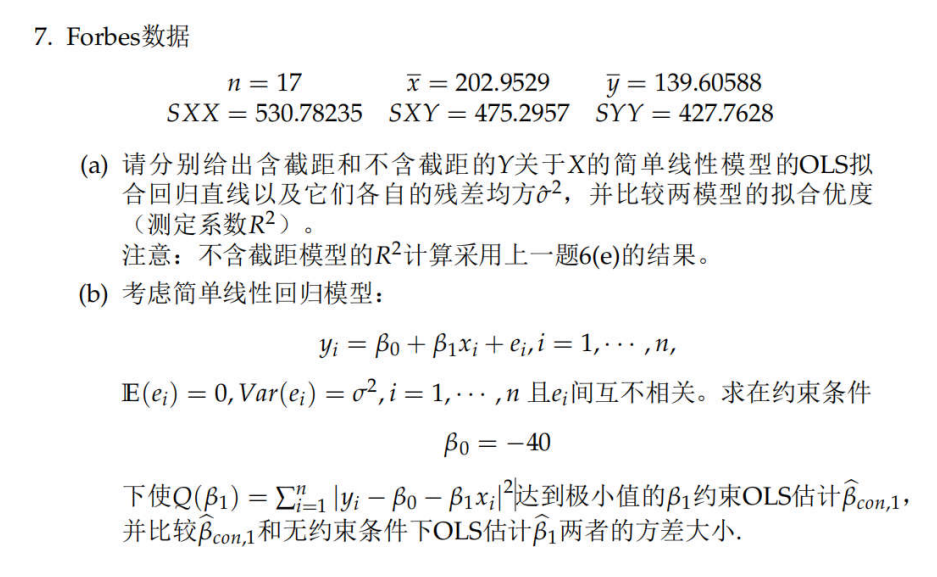
\includegraphics[width=30em]{image/ex2_plt7.png}
    \end{figure}

\begin{proof}[\solutionname]
(a)有截距模型:\[\hat{\beta_1}=\dfrac{SXY}{SXX}=0.895,\quad \hat{\beta_2}=\Bar{y}-\hat{\beta}_1\Bar{x}=-42.131\]
\[RSS = SYY-\dfrac{(SXY)^2}{SXX}=2.153,\quad \hat{\sigma}^2 = \dfrac{RSS}{n-2}=0.1435,\quad R^2 = \dfrac{(SXY)^2}{SXX\cdot SYY}=0.995
\]\[\hat{y}=-42.131+0.895x\]

无截距模型:\[\hat{\beta_1} = \dfrac{SXY+n\Bar{x}\Bar{y}}{SXX+n\Bar{x}^2}=0.688\]
\[RSS = SYY+n\Bar{y}^2-\dfrac{(SXY+n\Bar{x}\Bar{y})^2}{SXX+n\Bar{x}^2}=25.009 ,\quad \hat{\sigma}^2 = \dfrac{RSS}{n-1}=1.563,\quad \]
\[R^2 = \dfrac{(SXY+n\Bar{x}\Bar{y})^2}{(SXX+n\Bar{x}^2)(SYY+n\Bar{y}^2)}=0.9999,\quad \hat{y}=0.688x\]

无截距模型拟合优度较高。

\noindent (b)可以使用Lagrange乘子法,也可以在约束条件下求解新模型。这里将约束条件代入模型求解:
\[\hat{\beta}_{con,1}=\dfrac{\sum_{i=1}^n x_i(y_i+40)}{\sum_{i=1}^{n}x_i^2}=\dfrac{SXY+n\Bar{x}\Bar{y}+40n\Bar{x}}{SXX+n\Bar{x}^2}=0.885\]
\[var(\hat{\beta}_1)=\dfrac{\sigma^2}{SXX}\geq \dfrac{\sigma^2}{SXX+n\Bar{x}^2}=var(\hat{\beta}_{con,1})\]
\end{proof}

\begin{note}
    注意无截距模型中,$\hat{\sigma}^2=\frac{RSS}{n-1}$ % 此处答案将1.667改为1.563
\end{note}

\newpage
\begin{homework}
\end{homework}
    \begin{figure}[!htbp]
        \centering
        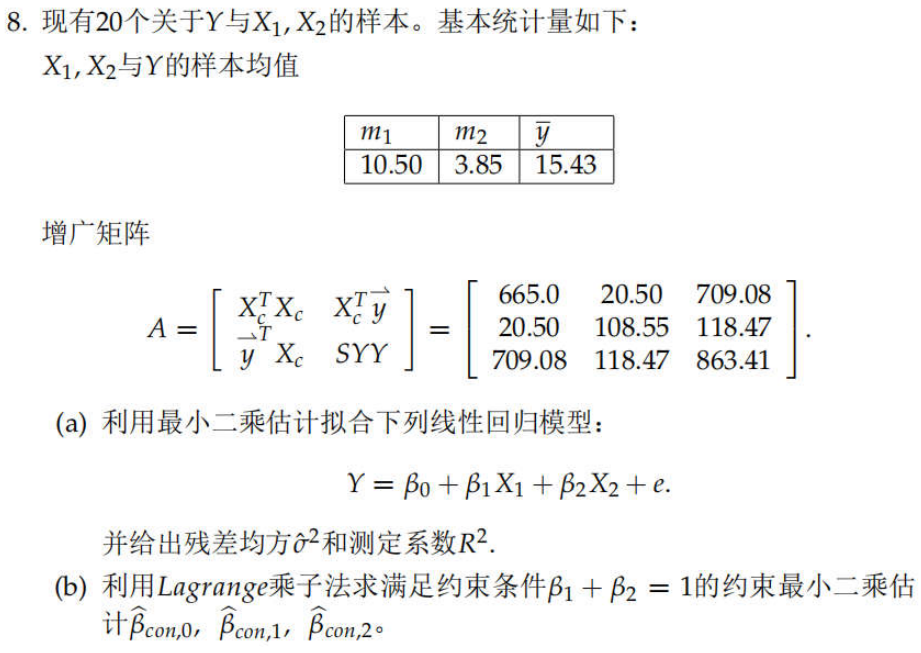
\includegraphics[width=30em]{image/ex2_plt10.png}
    \end{figure}

\begin{proof}[\solutionname]
(a) \[
\hat{\beta_c}=(X_c^TX_c)^{-1}X_c^Ty = \begin{bmatrix}
    1.039\\
    0.895\\ \end{bmatrix},\quad \hat{\beta}_0=\Bar{y}-(m_1, m_2)\hat{\beta}_c=1.0748
    \]
    回归方程
    \[\hat{y}=1.0748+1.039x_1+0.895x_2\]
    \[RSS = SYY-(y^TX_c)(X_c^TX_c)^{-1}(X_c^Ty) = 20.8, \quad \hat{\sigma}^2 = \frac{RSS}{n-3}=1.226\] 
\[R^2 = \dfrac{(y^TX_c)(X_c^TX_c)^{-1}(X_c^Ty)}{SYY} = \dfrac{SYY-RSS}{SYY}=0.9759\]

\noindent (b)
\[A = (1, 1)\; b = 1 \quad \hat{\beta}_{con}=\hat{\beta_c}-(X_c^TX_c)^{-1}A^T(A(X_c^TX_c)^{-1}A^T)^{-1}(A\hat{\beta_c}-b)\]
求解得
\[\hat{\beta}_{con} = \begin{bmatrix}
    0.9264\\
    0.0736\\
\end{bmatrix}=\begin{bmatrix}
    \hat{\beta}_{con,1}\\
    \hat{\beta}_{con,2}
\end{bmatrix},\quad \hat{\beta}_{con,0} = \Bar{y}-(m_1, m_2)\hat{\beta}_{con}=5.4192\]

\end{proof}


\begin{note}
    注意多步计算时,确保中间结果精度较高(保留四位小数),或者直接计算最后结果。
\end{note}
\newpage
\begin{homework}
\end{homework}
        \begin{figure}[!htbp]
        \centering
        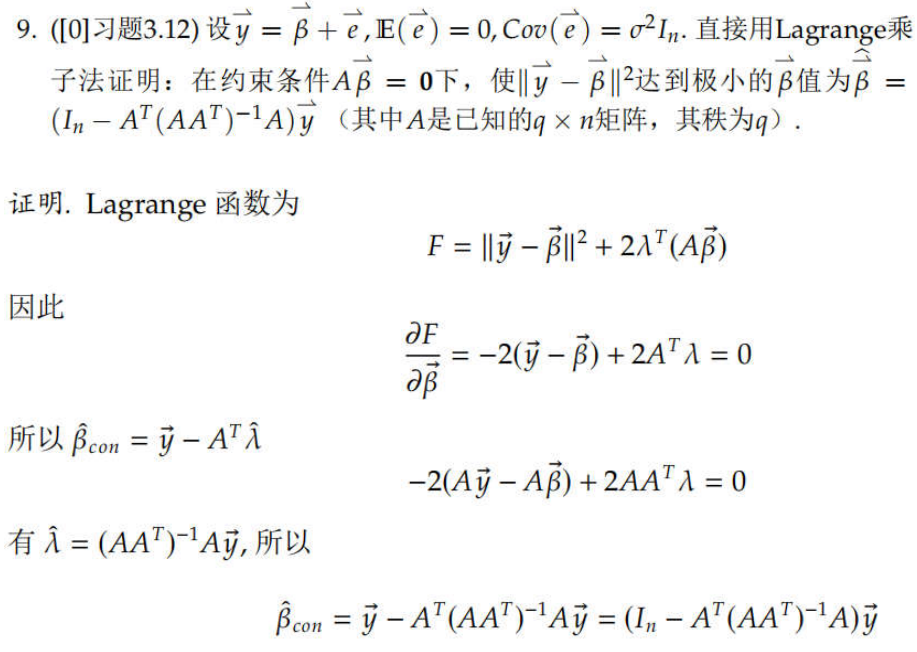
\includegraphics[width=30em]{image/ex2_plt13.png}
    \end{figure}

\begin{note}
    几何意义相当于求解$\bm y$在$A$的零空间中投影。注意到$N(A)=C(A^T)^{\perp}$,故
    \[\hat{\bm \beta}_{con} = P_{N(A)} \bm y=(I-P_{A^T})\bm y=(I-A^T(AA^T)^{-1}A)\bm y\]
\end{note}
\end{document}